\documentclass[UTF8]{ctexart}
\usepackage{geometry}
\usepackage{anyfontsize}
%\usepackage[fontsize=10pt]{fontsize}
\usepackage{amsmath}
\usepackage{amssymb}
\usepackage{mathtools}
\usepackage{mathrsfs}
\usepackage{ntheorem}
\usepackage{xcolor}
\usepackage{bm}
\usepackage{listings}
\usepackage{graphicx}
\usepackage{booktabs}
\usepackage[ruled,linesnumbered]{algorithm2e}

\geometry{margin=1.2in}

\DeclareMathOperator*{\argmax}{\arg\!\max}
\DeclareMathOperator*{\argmin}{\arg\!\min}

\newtheorem{theorem}{定理}[section]
\newtheorem{corollary}[theorem]{推论}
\newtheorem{lemma}[theorem]{引理}
\newenvironment{proof}{{\textit{证明}:\quad }}{\hfill $\blacksquare$\par}

\renewcommand{\algorithmcfname}{算法}
\SetKwInOut{KwIn}{输入}
\SetKwInOut{KwOut}{输出}
\SetNlSty{bfseries}{\color{black}}{}
\newcommand\mycommfont[1]{\footnotesize\ttfamily\textcolor{darkgray}{#1}}
\SetCommentSty{mycommfont}

\begin{document}

\title{流形优化期末报告}
\author{张晨}
\date{2024年9月23日}
\maketitle

\section{Question 1}

编程实现Algorithm 10和Algorithm 11. 下载文再文老师的代码. 运行文老师的代码, 比较简化版与ARNT, 指出文老师方法的优势. 

\subsection{数值实验比较}

首先, 我们使用文再文老师原论文中的非线性特征值问题(Single Nonlinear Eigenvalue Problems)为例, 从简化版算法与ARNT在这个优化问题的表现上出发, 比较两个算法的计算效果. 

考虑优化问题
\[\min_{X\in\mathbb{R}^{n\times p}} \frac{1}{2} \textup{tr}(X^T LX)+\frac{\alpha}{4}\rho(X)^T L^{-1}\rho(X),\quad\textup{subject to }X^T X=I_k.\]
其中$L$为一维Laplace算子离散化, 主对角线上全为$2$, 次对角线上全为$1$. $\rho(X)$是一个向量, 定义为$\rho(X)=\textup{diag}(XX^T)$. $\alpha$为一个常数. 我们使用Algorithm 11和ARNT对这个问题进行求解. 在参数选择上, 我们使用表\ref{tab2}中的参数值. 

\begin{table}[htb]
    \centering
    \begin{tabular}{c|cc}
        \hline
        \hline
        参数 & 具体数值 & 参数描述\\
        \hline
        $\sigma$ & $10$ & 初始正则参数\\
        $\gamma$ & $0.2$ & 回退幅度\\
        $c$ & $0.001$ & Armijo条件的系数\\
        $\eta_1$ & $0.01$ & 正则化调整下限参数\\
        $\eta_2$ & $0.09$ & 正则化调整上限参数\\
        $\gamma_1$ & $0.2$ & 正则化缩小幅度\\
        $\gamma_2$ & $10$ & 正则化增大幅度\\
        $\kappa$ & $0.01$ & 修正共轭梯度法偏差阈值\\
        method & Cayley变换 & 收缩映射方式\\
        $\varepsilon$ & $10^{-5}$ & 梯度阈值\\
        \hline
        \hline
    \end{tabular}
    \caption{算法参数}\label{tab2}
\end{table}

对于参数$n$, $p$和$\alpha$, 我们固定其中两个参数, 改变第三个参数, 进行数值实验, 得到结果分别见表\ref{tab3}, \ref{tab4}和\ref{tab5}, 其中的迭代数指正则化牛顿法的迭代次数, 总迭代数指修正共轭梯度法的总迭代次数.  

\begin{table}[htb]
    \centering
    \begin{tabular}{|c|cccc|cccc|}
        \hline
         & \multicolumn{4}{|c|}{Algorithm 11} & \multicolumn{4}{|c|}{ARNT}\\
        \hline
        n & 迭代数 & 总迭代数 & 梯度范数 & 时间 & 迭代数 & 总迭代数 & 梯度范数 & 时间\\
        \hline
        2000 & 8 & 146 & 1.18e-05 & 1.23 & 3 & 95 & 1.21e-05 & 0.47 \\
        \hline
        3000 & 8 & 154 & 6.23e-06 & 2.58 & 3 & 95 & 2.08e-05 & 0.84 \\
        \hline 
        5000 & 8 & 157 & 4.96e-06 & 5.92 & 4 & 121 & 2.47e-05 & 1.57 \\
        \hline
        8000 & 8 & 157 & 5.06e-06 & 12.37 & 3 & 100 & 1.29e-05 & 2.60 \\
        \hline 
        10000 & 8 & 167 & 2.77e-06 & 18.95 & 3 & 117 & 3.15e-06 & 3.43 \\
        \hline
    \end{tabular}
    \caption{$(p,\alpha)=(30,10)$时的数值实验结果}\label{tab3}
\end{table}

\begin{table}[htb]
    \centering
    \begin{tabular}{|c|cccc|cccc|}
        \hline
         & \multicolumn{4}{|c|}{Algorithm 11} & \multicolumn{4}{|c|}{ARNT}\\
        \hline
        p & 迭代数 & 总迭代数 & 梯度范数 & 时间 & 迭代数 & 总迭代数 & 梯度范数 & 时间\\
        \hline
        10 & 8 & 43 & 6.01e-05 & 3.51 & 3 & 32 & 3.85e-07 & 0.21 \\
        \hline
        20 & 8 & 106 & 4.73e-06 & 3.97 & 3 & 66 & 3.70e-06 & 0.70 \\
        \hline 
        30 & 8 & 157 & 4.96e-06 & 5.80 & 4 & 121 & 2.47e-05 & 1.60 \\
        \hline
        50 & 8 & 248 & 2.22e-05 & 9.60 & 3 & 180 & 3.28e-05 & 4.30 \\
        \hline 
    \end{tabular}
    \caption{$(n,\alpha)=(5000,10)$时的数值实验结果}\label{tab4}
\end{table}

\begin{table}[htb]
    \centering
    \begin{tabular}{|c|cccc|cccc|}
        \hline
         & \multicolumn{4}{|c|}{Algorithm 11} & \multicolumn{4}{|c|}{ARNT}\\
        \hline
        $\alpha$ & 迭代数 & 总迭代数 & 梯度范数 & 时间 & 迭代数 & 总迭代数 & 梯度范数 & 时间\\
        \hline
        1 & 10 & 107 & 8.00e-05 & 6.73 & 3 & 73 & 1.11e-06 & 1.87 \\
        \hline
        10 & 8 & 157 & 4.96e-06 & 5.61 & 4 & 121 & 2.47e-05 & 1.61 \\
        \hline 
        100 & 8 & 170 & 1.88e-06 & 5.96 & 4 & 108 & 7.00e-06 & 2.02 \\
        \hline
    \end{tabular}
    \caption{$(n,p)=(5000,30)$时的数值实验结果}\label{tab5}
\end{table}

从这些结果中可以看出, 对于实验中的这些例子, Algorithm 11的迭代数几乎都是$8$, ARNT的迭代数几乎都是$3$. 不过, 这些结果仍然揭示了一些信息: 
\begin{itemize}
    \item 当参数$n$增大时, 共轭梯度法的迭代次数没有明显差异, 但算法花费的时间增大了. 
    \item 当参数$p$增大时, 共轭梯度法的迭代次数和算法花费的时间都增大了. 
    \item 当参数$\alpha$增大时, 算法花费的时间没有明显的变化, 共轭梯度法的迭代次数的在$\alpha$较小时上升, 而在$\alpha$较大时保持基本不变. 
    \item Algorithm 11的表现在各方面都要差于ARNT. 
\end{itemize}

\subsection{修正共轭梯度法比较}

本小节中, 我们对简化版ARNT中使用的修正共轭梯度法Algorithm 10与ARNT中使用的修正共轭梯度法RNewton进行比较, 说明ARNT相比简化版的优点所在. 

首先, 我们将两个算法同时给出, 见算法\ref{algo1}和算法\ref{algo2}, 对于其中不同的部分, 我们使用不同的颜色加以区分, 其中绿色表示仅在这个算法中出现的部分, 红色表示在两个算法中都有出现, 但有所区别的部分. 为了更直观地展现两个算法的不同之处, 下面的伪代码将与书上和论文中的伪代码略有不同. 

\begin{algorithm}[htb]
    \caption{Algorithm 10}\label{algo1}
    \KwIn{黎曼梯度方向$g$, 黎曼海森算子$B$, {\color{teal}{偏差阈值$\kappa$}}}
    \KwOut{方程的解$d$, 其中方程为$Bd=-g$}
    {\color{teal}{$\varepsilon\leftarrow\min\big(0.5, \sqrt{\lVert g\rVert}\big)\lVert g\rVert$}};\quad$z_0\leftarrow 0$;\quad$r_0\leftarrow -g$;\quad$p_0\leftarrow -g$\tcp*{初始设置}
    \For{$j=0,1,2,\cdots$}{
        \If{{\color{purple}{$\langle p_j,Bp_j\rangle\leq 0$}}}{
            若$j=0$则$d\leftarrow -g$, 否则{\color{purple}{$d\leftarrow z_j$}}, 终止循环\tcp*{前进方向为零或负曲率方向}
        }
        $\alpha_j\leftarrow \frac{\langle r_j,r_j\rangle}{\langle p_j,Bp_j\rangle}$;\quad$z_{j+1}\leftarrow z_j+\alpha_j p_j$;\quad$r_{j+1}\leftarrow r_j-\alpha_j Bp_j$\tcp*{方程近似解更新}
        {\color{teal}{\If{$\langle z_{j+1},-g\rangle\le \kappa\lVert g\rVert\lVert z_{j+1}\rVert$}{
            $d\leftarrow z_j$, 终止循环\tcp*{方程近似解偏离负梯度方向}
        }}}
        \If{{\color{purple}{$\lVert r_{j+1}\rVert \le \varepsilon$}}}{
            $d\leftarrow z_{j+1}$, 终止循环\tcp*{残差很小}
        }
        $\beta_j\leftarrow \frac{\langle r_{j+1},r_{j+1}\rangle}{\langle r_j,r_j\rangle}$;\quad$p_{j+1}\leftarrow r_{j+1}+\beta_j p_j$\tcp*{解的前进方向更新}
    }
\end{algorithm}

\begin{algorithm}[htb]
    \caption{RNewton}\label{algo2}
    \KwIn{黎曼梯度方向$g$, 黎曼海森算子$B$, {\color{teal}{参数$T,\theta,\epsilon$}}}
    \KwOut{方程的解$d$, 其中方程为$Bd=-g$}
    $z_0\leftarrow 0$;\quad$r_0\leftarrow -g$;\quad$p_0\leftarrow -g$\tcp*{初始设置}
    \For{$j=0,1,2,\cdots$}{
        \If{{\color{purple}{$-\epsilon \langle p_j,p_j\rangle\leq \langle p_j,Bp_j\rangle\leq \epsilon \langle p_j,p_j\rangle$}}}{
            若$j=0$则$d\leftarrow -g$, 否则$d\leftarrow z_j$, 终止循环\tcp*{前进方向为零曲率方向}
        }
        \If{{\color{purple}{$\langle p_j,Bp_j\rangle\leq -\epsilon \langle p_j,p_j\rangle$}}}{
            若$j=0$则$d\leftarrow -g$, 否则{\color{purple}{$d\leftarrow z_j+\frac{\langle p_j,g\rangle}{\langle p_j,Bp_j\rangle} p_j$}}, 终止循环\tcp*{前进方向为负曲率方向}
        }
        $\alpha_j\leftarrow \frac{\langle r_j,r_j\rangle}{\langle p_j,Bp_j\rangle}$;\quad$z_{j+1}\leftarrow z_j+\alpha_j p_j$;\quad$r_{j+1}\leftarrow r_j-\alpha_j Bp_j$\tcp*{方程近似解更新}
        \If{{\color{purple}{$\lVert r_{j+1}\rVert \le\min(\lVert r_{0}\rVert^{\theta},T)$}}}{
            $d\leftarrow z_{j+1}$, 终止循环\tcp*{残差很小}
        }
        $\beta_j\leftarrow \frac{\langle r_{j+1},r_{j+1}\rangle}{\langle r_j,r_j\rangle}$;\quad$p_{j+1}\leftarrow r_{j+1}+\beta_j p_j$\tcp*{解的前进方向更新}
    }
\end{algorithm}

从算法\ref{algo1}和算法\ref{algo2}中可以直观地看出, 这两个算法的方程近似解更新和前进方向更新阶段是完全一样的, 不同点在于输入值、初始设置和跳出循环的方式, 而其中输入值和初始设置的不同是由于二者跳出循环的方式不同而导致的. 因此, 我们主要探讨二者跳出循环方式的差别. 

算法\ref{algo1}中跳出循环一共有三种方式: 前进方向成为零曲率或负曲率方向、近似解偏离负梯度方向、方程的残差很小; 算法\ref{algo2}中跳出循环一共有两种方式: 前进方向成为零曲率或负曲率方向、方程的残差很小. 对于第一种跳出方式, 算法\ref{algo1}并没有对零曲率和负曲率方向进行区分, 而算法\ref{algo2}对零曲率方向和负曲率方向进行了分类, 给出了不同的算法输出. 

\subsection{正则化牛顿法比较}

在上一节中我们已经比较过了Algorithm 10与RNewton算法之间的不同点. 在本节中, 我们用同样的的方式比较Algorithm 11与ARNT算法之间的不同点, 两个算法的伪代码实现见算法\ref{algo3}和算法\ref{algo4}, 其中的$f$为待优化函数, $m_k$为$f$在$x_k$点二阶展开后正则化的近似模型
\[m_k(d)=f(x_k)+\langle \textup{grad}f(x_k),d\rangle+\frac{1}{2}\langle \textup{Hess}f(x_k)d,d\rangle+\frac{\sigma_k}{2}\lVert d\rVert^2.\]

\begin{algorithm}[htb]
    \caption{Algorithm 11}\label{algo3}
    \KwIn{初始点$x_0$, 初始参数$\sigma_0$, 系数$c$, 回退幅度$\gamma$, 正则阈值$\eta_1,\eta_2$, {\color{purple}{正则幅度$\gamma_1,\gamma_2$}}}
    $k\leftarrow 0$\;
    \While{终止条件不成立}{
        {\color{purple}{使用Algorithm 10}}得到步长$d_k$\;
        初始步长为$1$, 使用{\color{purple}{关于$f$}}的回退法线搜索得到步长$t_k$和中间点$y_k=\textbf{R}_{x_k}(t_kd_k)$\;
        计算预测比$\rho_k\leftarrow\frac{f(y_k)-f(x_k)}{m_k(t_k d_k)-f(x_k)}$\;
        更新正则参数: 若$\rho_k\geq \eta_2$, 则{\color{purple}{$\sigma_{k+1}\leftarrow\gamma_1\sigma_k$}}; 若$\eta_2\ge\rho_k\geq \eta_1$, 则{\color{purple}{$\sigma_{k+1}\leftarrow\sigma_k$}}; 若$\rho_k\le \eta_1$, 则{\color{purple}{$\sigma_{k+1}\leftarrow\gamma_2\sigma_k$}}\; 
        更新迭代点: 若$\rho_k\geq \eta_1$, 则$x_{k+1}\leftarrow y_k$; 若$\rho_k\le \eta_1$, 则$x_{k+1}\leftarrow x_k$\; 
        $k\leftarrow k+1$\;
    }
\end{algorithm}

\begin{algorithm}[htb]
    \caption{ARNT}\label{algo4}
    \KwIn{初始点$x_0$, 初始参数$\sigma_0$, 系数$c$, 回退幅度$\gamma$, 正则阈值$\eta_1,\eta_2$, {\color{purple}{正则幅度$\gamma_0,\gamma_1,\gamma_2$}}}
    $k\leftarrow 0$\;
    \While{终止条件不成立}{
        {\color{purple}{使用RNewton}}得到步长$d_k$\;
        初始步长为$1$, 使用{\color{purple}{关于$m_k$}}的回退法线搜索得到步长$t_k$和中间点$y_k=\textbf{R}_{x_k}(t_kd_k)$\;
        计算预测比$\rho_k\leftarrow\frac{f(y_k)-f(x_k)}{m_k(t_k d_k)-f(x_k)}$\;
        更新正则参数: 若$\rho_k\geq \eta_2$, 则{\color{purple}{$\sigma_{k+1}\in(0,\gamma_0\sigma_k]$}}; 若$\eta_2\ge\rho_k\geq \eta_1$, 则{\color{purple}{$\sigma_{k+1}\in[\gamma_0\sigma_k,\gamma_1\sigma_k]$}}; 若$\rho_k\le \eta_1$, 则{\color{purple}{$\sigma_{k+1}\in[\gamma_1\sigma_k,\gamma_2\sigma_k]$}}\; 
        更新迭代点: 若$\rho_k\geq \eta_1$, 则$x_{k+1}\leftarrow y_k$; 若$\rho_k\le \eta_1$, 则$x_{k+1}\leftarrow x_k$\; 
        $k\leftarrow k+1$\;
    }
\end{algorithm}

从算法\ref{algo3}和算法\ref{algo4}可以看出, Algorithm 11与ARNT的区别主要在两点: 其一, Algorithm 11使用的是关于$f$的回退法线搜索, 而ARNT使用的是关于$m_k$的回退法线搜索; 其二, 二者的正则化参数更新过程不同. 

\section{Question 2}

编程实现教材上的Algorithm 3和Algorithm 4, 随机生成Stiefel流形的一个二次函数, 用Algorithm 4极小化这个二次函数, 比较两个算法的计算效果, 探索非单调的作用, 或者交替使用BB步长两个公式的作用. 

\subsection{随机二次函数的生成}

首先考虑实现二次函数的随机生成问题. 对于整数$n\geq p>0$, 欧氏空间$\mathbb{R}^{n\times p}$上的$Stiefel$流形为
\[\textup{St}(n,p)=\{X\in\mathbb{R}^{n\times p}|X^T X=I_p\}.\]
对于矩阵$B\in \mathbb{R}^{n\times p}$和对称正定矩阵$A\in\mathbb{R}^{n\times n}$, $St(n,p)$上的二次函数定义为
\[f(X;A,B)=\textup{tr}(X^T AX+2X^T B).\]
故二次函数$f$的生成问题等价于矩阵$A,B$的生成问题. 在MATLAB中, 可以使用\textbf{randn}函数随机生成矩阵, 因此, 可以取
\[B\leftarrow \textup{randn}(n,p).\]
但MATLAB中并没有直接生成对称正定矩阵的函数. 为了随机生成$A$, 先考虑一个简单的引理: 
\begin{lemma}
    记集合$\mathcal{A}$为对称正定矩阵全体, 定义集合
    \[\mathcal{B}=\{R^T R+D|R\in\mathbb{R}^{n\times n}, D=\textup{diag}(d_1,\cdots,d_n), 0<d_1,\cdots,d_n<1\},\]
    则$\mathcal{A}=\mathcal{B}$. 
\end{lemma}
\begin{proof}
    首先证明$\mathcal{B}\subseteq\mathcal{A}$. 对于任意的$B=R^T R+D\in\mathcal{B}$, 有
    \[B^T=(R^T R+D)^T=R^T R+D^T=R^T R+D=B,\]
    故$B$是对称的. 对于任意的$x\in\mathbb{R}^n_*$, 有
    \[x^T Bx=(Rx)^T(Rx)+x^T Dx\geq x^T Dx\geq d_1 \lVert x \rVert_2^2>0.\]
    因此, $B\in\mathcal{A}$.

    再证明$\mathcal{A}\subseteq\mathcal{B}$. 对于任意的$A\in\mathcal{A}$, 记$\lambda>0$为$A$的最小特征值, 取$d=\min(\lambda/2,1/2)$, 则矩阵$A-dI_n$仍为对称正定矩阵. 注意到, 根据对称正定矩阵的Cholesky分解, 存在矩阵$R\in\mathbb{R}^{n\times n}$, 使得
    \[A=(A-dI_n)+dI_n=R^T R+dI_n\in\mathcal{B}.\]
    综上, $\mathcal{A}=\mathcal{B}$. 
\end{proof}

根据这个引理, 结合MATLAB中取值在$(0,1)$上的随机函数\textbf{rand}, 可以得到对称正定矩阵的随机生成方法:
\begin{align*}
    R&\leftarrow \textup{randn}(n,n),\\
    A&\leftarrow R^T R+\textup{diag}(\textup{rand}(n)). 
\end{align*}

详细的代码实现可以参考附录. 在下文中, 我们考虑$n=500$, $p=50$时各算法的表现, 取MATLAB中随机函数的种子为$99$, 生成的矩阵对$(A,B)$同样可见附录.

\subsection{梯度下降算法与BB算法的比较}

本小节中, 我们使用基于单调线搜索的梯度下降算法与基于非单调线搜索的BB算法对二次函数$f(X)=\textup{tr}(X^T AX+2X^T B)$进行优化. 在参数选择上, 我们使用表\ref{tab1}中的参数值. 

\begin{table}[htb]
    \centering
    \begin{tabular}{c|cc}
        \hline
        \hline
        参数 & 具体数值 & 参数描述\\
        \hline
        $t_0$ & $0.02$ & 回退法的初始步长\\
        $\rho$ & $0.5$ & 回退幅度\\
        $c$ & $0.001$ & Armijo条件的系数\\
        $M$ & $5$ & 非单调线搜索的前项个数\\
        $\alpha_{\max}$ & $100$ & BB步长的上界\\
        $\alpha_{\min}$ & $0.01$ & BB步长的下界\\
        method & QR分解 & 收缩映射算法\\
        \hline
        \hline
    \end{tabular}
    \caption{算法参数}\label{tab1}
\end{table}

我们先分析一下两个算法的收敛速度, 随机选取初始点$X_0$, 观察函数值$f(X_k)$与点列$X_k$的误差变化情况, 结果见图\ref{fig1}, 其中左图为函数值$f(X_k)$的相对误差随迭代次数的变化情况, 右图为自变量点列$X_k$关于极小值点$X^*$的相对误差, 其度量为两点作为$\mathbb{R}^{n\times p}$矩阵时, 差值$X_k-X^*$的Frobenius范数. 

\begin{figure}[htb]
    \centering
    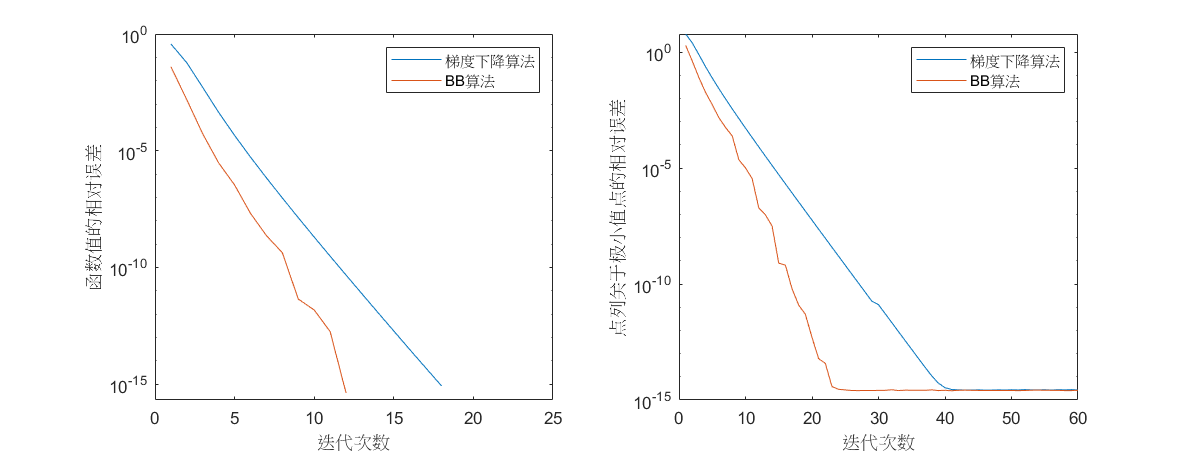
\includegraphics[width=0.7\textwidth]{Q2-figure/1.png}
    \caption{相对误差的变化情况}\label{fig1}
\end{figure}

从图\ref{fig1}中可以看出: 首先, 两个算法都在$50$步内迭代到了最小值点, 误差达到了机器精度; 其次, 这两个算法的收敛速度都是线性收敛, 且BB算法的速度要显著快于梯度下降算法; 最后, 函数值的收敛速度比自变量点列的收敛速度更快, 这一点是由二次函数的性质产生的. 

接下来, 对于不同的收缩映射算法, 我们对比一下算法的收敛速度, 结果见图\ref{fig2}, 其中左图均为函数值的相对误差变化情况, 右图均为自变量点列的相对误差变化情况, 第一行为使用梯度下降算法得到的误差变化图, 第二行为使用BB算法得到的误差变化图. 

\begin{figure}[htb]
    \centering
    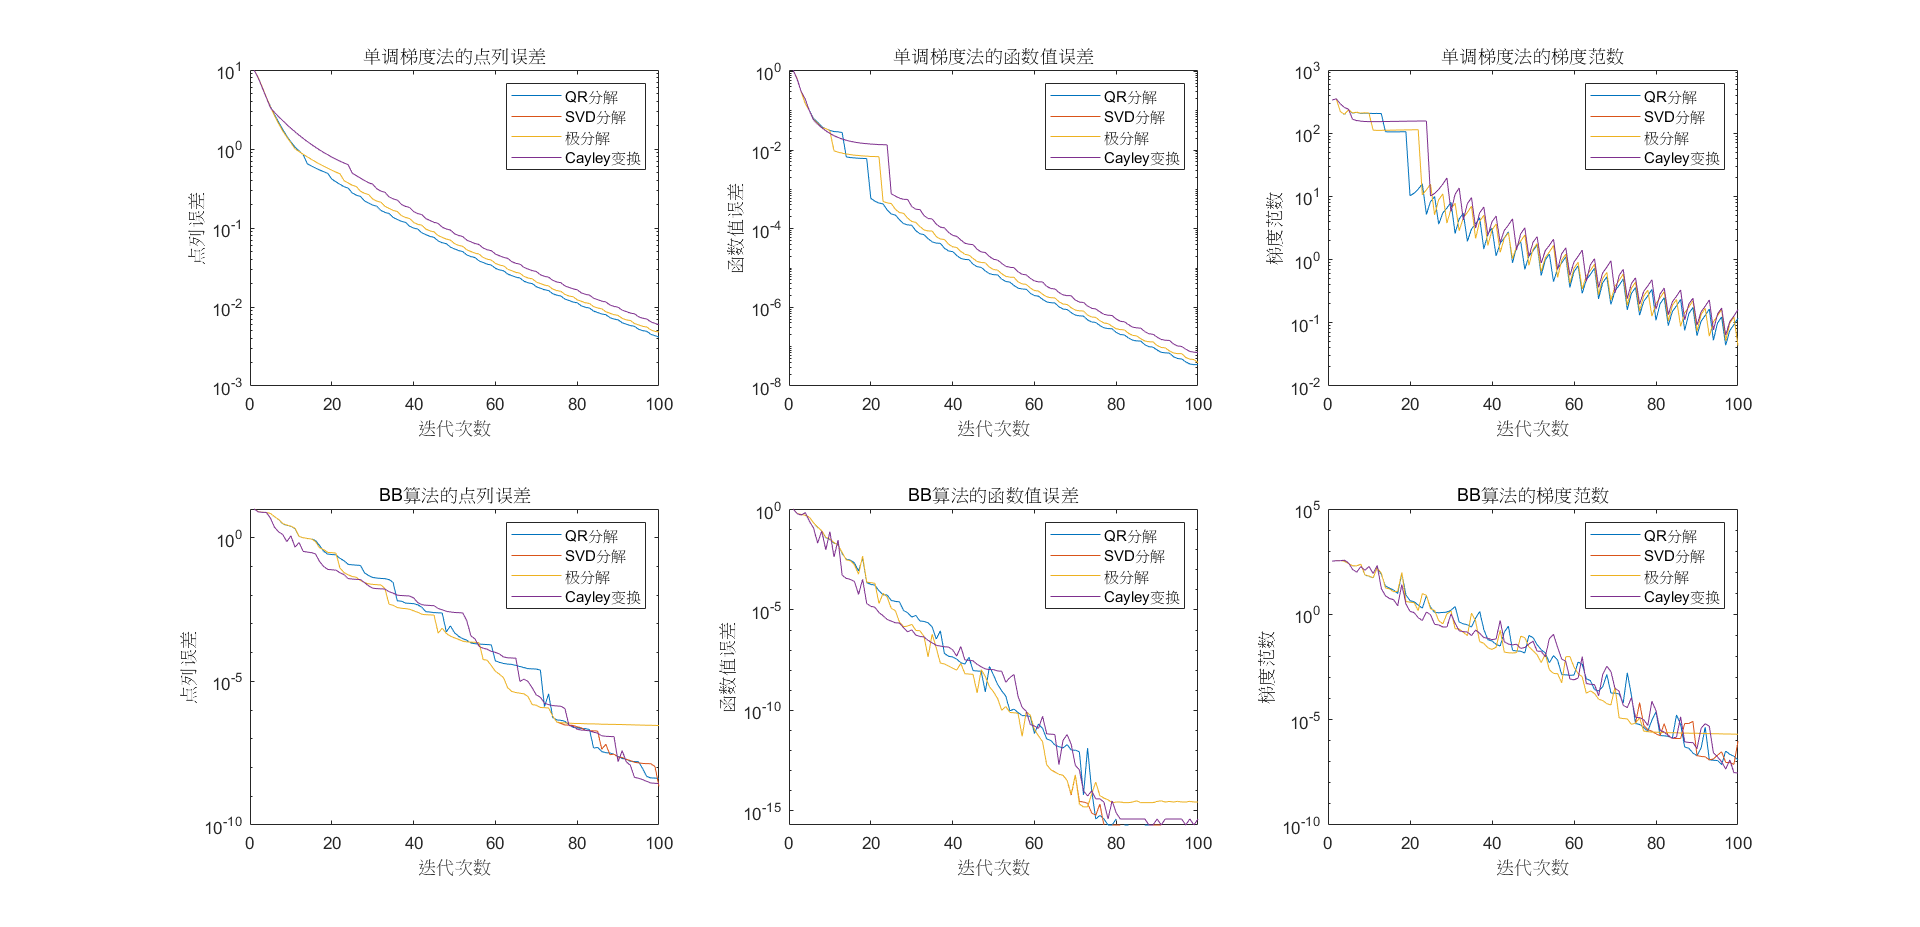
\includegraphics[width=0.7\textwidth]{Q2-figure/2.png}
    \caption{不同收缩映射算法的表现}\label{fig2}
\end{figure}

从图\ref{fig2}中可以看到, 不同收缩映射算法在函数值上的表现是相同的, 以同样的速度线性收敛. 值得一提的是, 基于Cayley变换的收缩映射算法会导致BB算法在前几次迭代的效果略差, 但在之后的迭代中仍然获得了和其他收缩映射算法相同的收敛速度. 当考察自变量$X$的收敛情况时, 不同的收缩映射算法产生了不同的表现. 在BB算法中, 基于Cayley变换的收缩映射算法仍然在前几次迭代中表现略差, 不过在长期迭代中, 这些收缩映射的表现是类似的; 但在梯度下降算法中, 基于QR分解和Cayley变换的收缩映射算法很快到达了机器精度, 基于SVD分解的收缩映射算法在20次迭代后放缓了收敛速度, 基于极分解的收缩映射算法只能达到$10^{-6}$精度, 无法达到机器精度. 

值得特别一提的是, 在理论上, 基于SVD分解的收缩映射和基于极分解的收缩映射应当是同一个, 但这两种不同的收缩映射在梯度下降算法下的表现是不同的, 这可能是计算误差导致的: 在实现基于SVD分解的收缩映射时, 我们直接使用了MATLAB内置的\textbf{svd}函数, 这一函数是使用商业库MKL构建的, 因此会进行专业的优化, 达到比极分解更好的表现. 

\subsection{非单调线搜索的作用}
本小节中, 我们通过使用不同的前项个数$M$对二次函数$f(X)$进行优化, 探索非单调线搜索的作用. 在正式讨论前, 先观察一个现象: 取初始步长$t_0=0.02$和$0.08$, 前项个数$M=5$, 其他参数同表\ref{tab1}, 查看单调线搜索与非单调线搜索的表现. 其结果见图\ref{fig3}, 其中左图为初始步长$t_0=0.02$时的表现, 右图为初始步长$t_0=0.08$时的表现, 图像为函数值的相对误差随迭代次数的变化情况, Armijo条件指单调线搜索, Grippo条件指Grippo提出的非单调线搜索, 凸组合条件指H. Zhang与W. W. Hager提出的非单调线搜索, 其系数$\varrho=0.5$. 

\begin{figure}[htb]
    \centering
    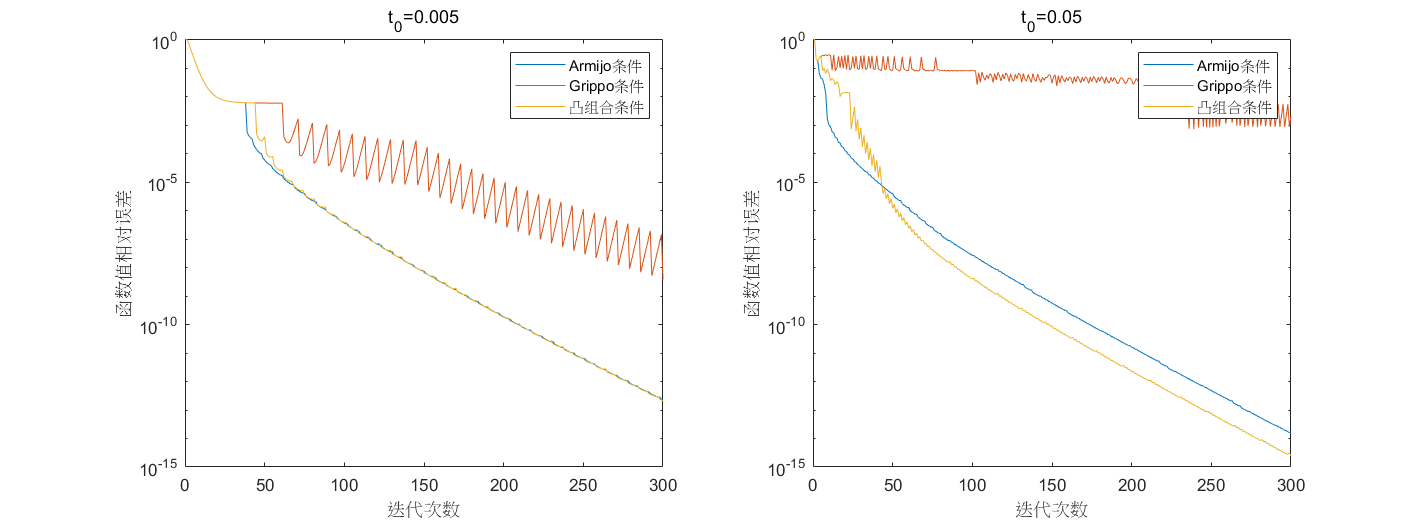
\includegraphics[width=0.7\textwidth]{Q2-figure/3.png}
    \caption{步长对函数值误差的影响}\label{fig3}
\end{figure}

从图\ref{fig3}中可以看到, 当初始步长$t_0=0.02$时, 单调线搜索与非单调线搜索都在很少的迭代步数中达到了非常低的误差, 但当初始步长$t_0$提高$4$倍, 变成$0.08$后, 单调线搜索的收敛速度没有降低, 但非单调线搜索的表现大大降低了, 凸组合线搜索在更多的迭代步数后才能达到同样的误差, 而Grippo线搜索的收敛速度变得非常缓慢. 一种可能的解释是, Grippo条件比Armijo条件和凸组合条件更宽松, 这导致算法在接近最小值点、初始步长很大时容易越过最小值点而跳到更远的地方, 导致下降缓慢. 

大步长造成的影响并非仅限于Grippo线搜索, 事实上, 大步长对每一个梯度下降算法都造成了影响. 为了说明这一点, 我们来查看不同初始步长下自变量$X$的收敛情况, 所有参数同上, 结果见图\ref{fig4}. 

\begin{figure}[htb]
    \centering
    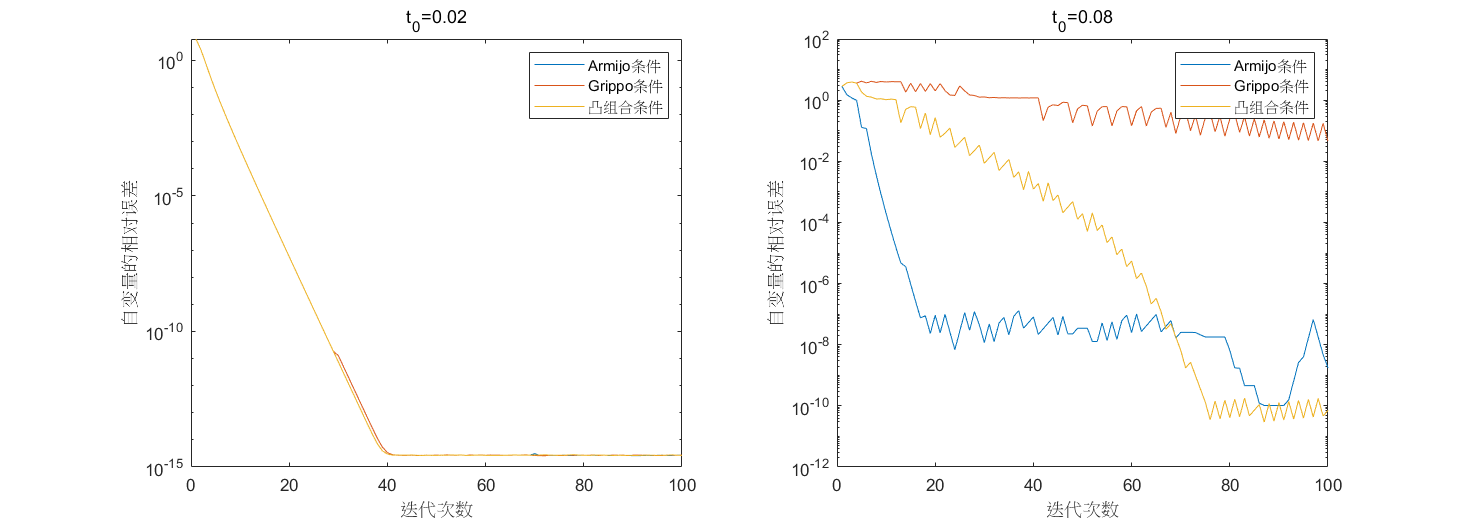
\includegraphics[width=0.7\textwidth]{Q2-figure/4.png}
    \caption{不同步长下自变量误差的变化}\label{fig4}
\end{figure}

从图\ref{fig4}中可以看到, 当初始步长$t_0=0.02$时, 所有算法都在$40$步内迭代到了机器误差. 当初始步长变为$0.08$后, Grippo线搜索不出所料没有收敛, 但单调线搜索与凸组合线搜索的误差也变大了, 凸组合线搜索的误差维持在了$10^{-10}$, 而单调线搜索更是只能达到$10^{-8}$. 为了更直观地体现步长对自变量收敛值的影响, 我们使用不同的步长进行实验, 结果见图\ref{fig5}, 其中$x$轴为初始步长, $y$轴为迭代$1000$步后的自变量误差, 其余参数同上. 

\begin{figure}[htb]
    \centering
    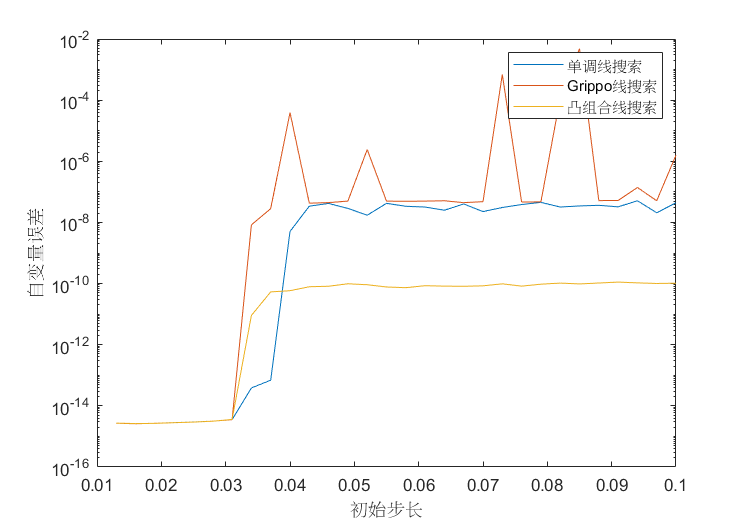
\includegraphics[width=0.4\textwidth]{Q2-figure/5.png}
    \caption{步长对自变量误差的影响}\label{fig5}
\end{figure}

从图\ref{fig5}中可以看到, 当初始步长$t_0\leq 0.03$时, 三个算法都能达到机器精度, 但当初始步长$t_0>0.03$时, 三个算法跳跃到了更大的误差上. 凸组合线搜索在大步长时, 自变量误差稳定在了$10^{-11}$上; 单调线搜索和Grippo线搜索只能达到$10^{-8}$量级的精度, 并且Grippo线搜索甚至在$1000$步后仍无法保证收敛, 误差有时会升到$10^{-3}$. 产生这种情况的原因仍不清楚, 有待更详细的实验与分析. 

现在我们正式考察不同参数$M$对梯度下降算法的影响, 取初始步长$t_0=0.02,0.1$, $M=1,3,5,7$, 其余参数同表\ref{tab1}, 结果见图\ref{fig6}. 

\begin{figure}[htb]
    \centering
    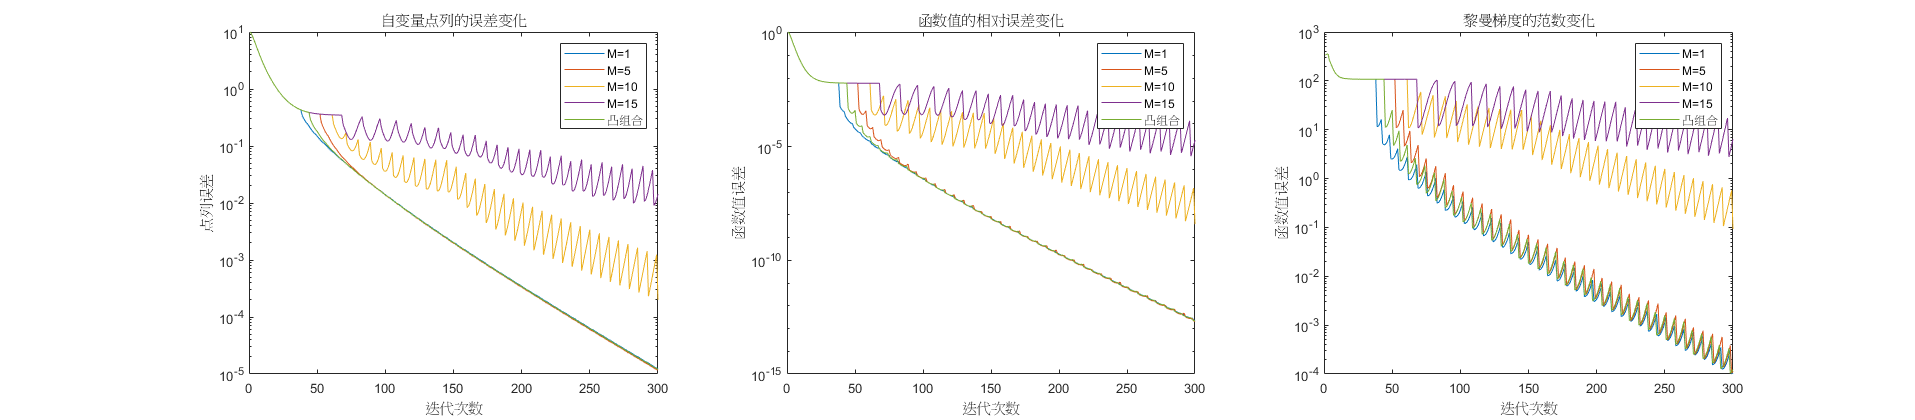
\includegraphics[width=0.7\textwidth]{Q2-figure/6.png}
    \caption{不同参数$M$下梯度下降法的表现}\label{fig6}
\end{figure}

从图\ref{fig6}中可以看到, 当初始步长$t_0=0.02$时, 不同的参数$M$带来的函数值变化和自变量变化是几乎完全一致的. 这可能是由于本问题中选取的矩阵$A$很好, 使得梯度下降法在很少的迭代次数后就达到了最小值点附近, 而初始步长又很小, 导致回退法并没有产生回退步骤, 进而让回退法的梯度下降法退化成了固定步长的梯度下降法, 因此这些算法并没有明显的区分. 当初始步长$t_0=0.1$时, 不同的参数$M$产生了不同的效果: 
\begin{itemize}
    \item 随着$M$的增大, 梯度下降法的收敛速度变得越来越慢.
    \item 随着$M$的增大, 函数值误差的波动也越来越大.
    \item $M=5$和$M=7$的收敛速度是一样的, 但$M=7$在算法前期更频繁地短暂停留在了某个点, 导致其需要花费更多的迭代次数才能达到合适的误差. 
    \item 相比于单调线搜索, 非单调线搜索的自变量误差要更稳定一些. 
    \item 凸组合线搜索的收敛速度要略慢于单调线搜索, 但收敛后凸组合线搜索的自变量误差要小于单调线搜索的自变量误差. 
\end{itemize}

对于第一点, 这有可能是因为本问题中的矩阵$A$性质很好, 因此单调线搜索就可以产生很好的效果, 而非单调线搜索反而因为更宽松的条件导致容易跑离最小值点; 对于第二点, 这是符合直观的, 因为单调线搜索可以保证函数值单调下降, 但非单调线搜索有可能使得函数值短暂上升, 并且$M$越大, 函数值的波动就越剧烈, 不过其总体上是下降的; 对于第三点, 这有可能说明在本问题中, $M$的不断增大并不会导致算法的收敛速度不断变慢, 而是有可能会使收敛速度达到一个下界, 不会继续降低; 第四点和第五点的产生原因仍有待更进一步的分析. 

\subsection{交替使用BB步长的作用}
本小节中, 我们探索一下交替使用BB步长的作用. 选取参数如下: $\alpha_{\max}=1000$, $\alpha_{\min}=0.001$, 初始步长$\alpha_0=0.02$, 其余参数同表\ref{tab1}, 我们直接考察使用交替步长、仅使用短BB步长、仅使用长BB步长这三种情况下BB算法的表现情况, 结果见图\ref{fig7}, 其中左图为函数值$f(X)$随迭代次数的相对误差变化, 中间为自变量$X$随迭代次数的相对误差变化, 右图为BB步长随迭代次数的相对误差变化. 

\begin{figure}[htb]
    \centering
    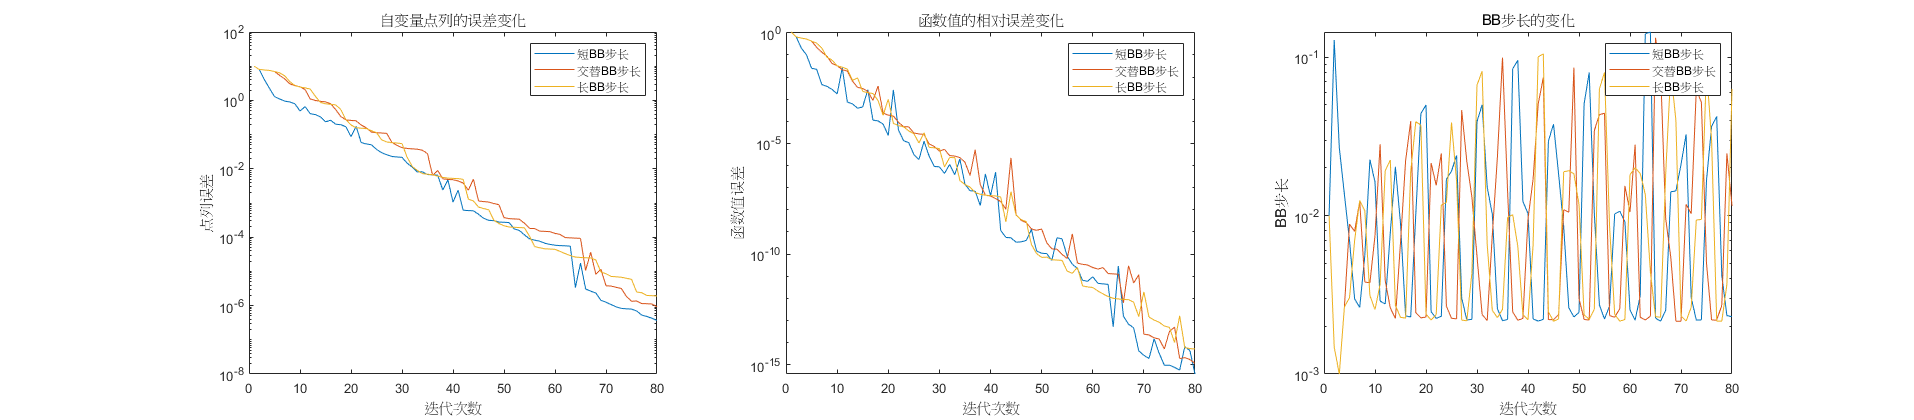
\includegraphics[width=\textwidth]{Q2-figure/7.png}
    \caption{不同BB步长的表现}\label{fig7}
\end{figure}

从图\ref{fig7}中可以看出, 在本问题中, 选择不同的BB步长并不会带来很大不同, 三种算法无论是在函数值$f(X)$还是在自变量$X$的误差变化上都非常相似. 这三种算法不同的是BB步长的表现, 当全程使用长BB步长时, 每一步的BB步长会略大于使用交替BB步长时的长BB步长, 同样, 全程使用短BB步长时, 每一步的BB步长会略小于使用交替BB步长时的短BB步长. 

\end{document}